%!TEX root = ../main.tex
%%%%%%%%%%%%%%%%%%%%%%%%%%%%%%%%%%
% Links:
%
% Difficulty: Companies: 
%%%%%%%%%%%%%%%%%%%%%%%%%%%%%%%%%%

\chapter{Largest square in a binary matrix}
% type of problem why can be useful in real life (image segmentation) dynamic programming
\label{ch:square_in_matrix}
\section*{Introduction}
Imagine you are given a black and white image represented as a boolean matrix of size $N\times M$
where $0$ and $1$ in the matrix correspond to a black and white pixel respectively. Such kind of
image are less uncommon that might be thought at first because they are often the output of digital
image processing algorithms such as masking or thresholding. Further analyzing this kind of images
often requires to identify homogeneous portions of the image. The problem described in this chapter
deals with a simple type of image processing algorithm that involves determining the size of the
largest square area of white pixel of a binary bitmap. We will walk through a number of solutions,
starting from a naive brute-force one, to a more sophisticated, more complex and definitely more
efficine one.
 

\section{Problem statement}
\begin{exercise}
Given a 2D boolean matrix $M$, return the area of the largest square containing only one cells.
	\begin{example}
		\hfill \\
		Given the following matrix the function returns $9$. The largest square has side lenght of
		$3$ and the coordinate of the top-left corner are $(2,1)$. Cells belonging to the largest
		square are highlighted.

		\begin{tabular}{|l|l|l|l|l|}
		\hline
		0 & 0                                  & 1                                  & 1 & 1 \\
		\hline
		0 & 0                                  & 1                                  & 1 & 0 \\
		\hline
		0 & \cellcolor[HTML]{32CB00}\textbf{1} & \cellcolor[HTML]{32CB00}\textbf{1} &
		\cellcolor[HTML]{32CB00}\textbf{1} & 0 \\ \hline
		1 & \cellcolor[HTML]{32CB00}\textbf{1} & \cellcolor[HTML]{32CB00}\textbf{1} &
		\cellcolor[HTML]{32CB00}\textbf{1} & 0 \\ \hline
		1 & \cellcolor[HTML]{32CB00}\textbf{1} & \cellcolor[HTML]{32CB00}\textbf{1} &
		\cellcolor[HTML]{32CB00}\textbf{1} & 0 \\ \hline
		\end{tabular}
		
	\end{example}

	\begin{example}
		\hfill \\
		Given the following matrix the function returns $4$. The side of the largest square is $2$
		and the top-left coordinates are $(2,2)$. Cells belonging to the largest square are
		highlighted.
		\begin{tabular}{|l|l|l|l|l|}
		\hline
		1 & 0 & 1                                  & 0                                  & 0 \\
		\hline
		1 & 0 & \cellcolor[HTML]{32CB00}\textbf{1} & \cellcolor[HTML]{32CB00}\textbf{1} & 1 \\
		\hline
		1 & 1 & \cellcolor[HTML]{32CB00}\textbf{1} & \cellcolor[HTML]{32CB00}\textbf{1} & 1 \\
		\hline
		1 & 0 & 0                                  & 1                                  & 0 \\
		\hline
\end{tabular}

	\end{example}

\end{exercise}


\section{Discussion}
\label{square_in_matrix:sec:discussion}
In the next section we will analyze a number of possible approaches to this problem. We start by
looking at a few brute-force approaches so to then move towards more elaborate and more time and
space efficient dynamic programming solutions

\subsubsection{Brute-force - Incremental side}
\label{square_in_matrix:sec:incremental_side}
The first brute-force approach consists of trying to find the largest square made entirely of set
(i.e. holding a value of $1$) cell by visiting each set cell and by treating it as if it was the
top-left corner of a square. Because calculating the largest square having that cell as top-left
corner is easy the answer to the problem is just the largest value over all the set cells in the matrix.
In order to find out what the value of the largest square having cell $(x,y)$ as top-left corner we
can try build squares of incrementally larger sides around it, starting from side lenght $1$. At
first we try to build a square of size $1$. If that is possible we try size $2$, then $3$, and so
on, until it is impossible or we hit the boundaries of the matrix. The answer for the cell $(x,y)$
is the last value for a side for which we were able to construct a square.
Consider for instance Figure \ref{fig:square_in_matrix:squa_matrix_incremental}
where in order to find the value of the largest square can be built from cell
$(0,1)$, all squares highlighted have to be fully checked.
This approach is clearly correct because eventually we find all squares in the matrix, and
has a complexity of (assuming, with no loss in generality, $N \leq M$) $O(N^4M)$. This is because
there are $O(NM)$ possible starting point for a square, $O(N)$ possible values
for the side value and checking whether a square is valid costs $O(N^2)$ (all cells in the square needs to be
checked). A possible implementation of this idea
is shown in the Listing \ref{list:square_in_matrix:bruteforce1}.


\lstinputlisting[language=c++, caption={Brute force soltuion solution to the \textit{square in matrix} problem using incremental side probing.},label=list:square_in_matrix:bruteforce1]{sources/square_in_matrix/square_in_matrix_solution1.cpp}

\begin{figure}
	\centering
	\label{fig:square_in_matrix:squa_matrix_incremental}
	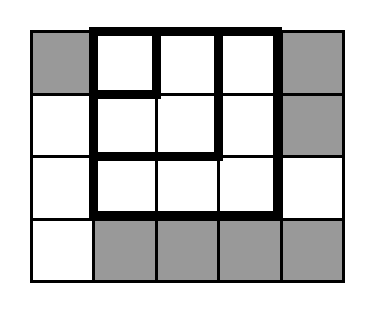
\includegraphics[width=\textwidth/2]{sources/square_in_matrix/images/squa_matrix_incremental}
	\caption[Square in matrix - Brute-force incremental square
	construction.]{This figure shows  the squares that are checked by the
	brute-force approach for solving the square in matrix problem. 
	From the cell $(0,1)$ we first try to build a square of side $2$, and when
	that is verified to be possible, a square of size $3$ is tried. This also
	succeed and so a square of side $4$ is checked, with a negative outcome.
	Thus $3$ is the largest square having cell $(0,1)$ as top left corner. }
\end{figure}

\subsubsection{Brute-force improved}
The idea presented in the Section \ref{square_in_matrix:sec:incremental_side} can be significantly
improved by noticing that is it really not necessary to check, given a cell
$(x,y)$ squares of all
possible side lenghts having it as top left corner, fully and one after the
other.
The idea is that we can walk diagonally (towards the bottom-right cell) from
$(x,y)$ (by incrementing both $x$ and $y$) and, for every step $i$ we take, we check whether all the
elements to the left of $(x+i, y+i)$  and to the right of  $y$ are set, and also whether all the
cells in the columns above $(x+i, y+i)$ and below the cell $(x,y+i)$ are set
(see Figure \ref{fig:square_in_matrix:squa_matrix_diagonal}). If both conditions are
true it means that we can construct a square of side $i$. We can then proceed
one step further until a $0$ is found among the checked cells on the left or
above.
If we were able to perform $t$ diagonal steps, it means we have found out that the largest square having $(x,y)$ as top-left corner has an
area of $t^2$. The final answer is the largest value we calculated this way across all cell that are
set. See Figure \ref{fig:square_in_matrix:squa_matrix_diagonal} where the
numbers represents the cells that are checked during the corrensponding step. Every highlighted square depicts
one of the squares that is checked by the algorithm.


The time complexity of this approach is $N^3M$, lower than the previous solution. As shown in
Section \ref{square_in_matrix:sec:incremental_side}, there are $NM$ potential top-left corner for a
square and for each of them $O(N)$ diagonal steps. Each diagonal steps costs $O(N)$ as in the worst
case we must check one entire row and column. Thus the complexity of calculating
the value of the largest square having a certain cell as top-left corner is
$O(N^2)$ (Figure \ref{fig:square_in_matrix:square_matrix_diagonal} shows that no
cell is checked twice). Listing \ref{list:square_in_matrix_diagonal} shows a
possible implementation of the idea described here. Note how
Listings \ref{list:square_in_matrix_diagonal} and
\ref{list:square_in_matrix:bruteforce1} for both the solutions proposed so far are very
similar, with the only difference being in how the largest
square constructible from a certain top-left cell is computed.

\begin{figure}
	\centering
	\label{fig:square_in_matrix:square_matrix_diagonal}
	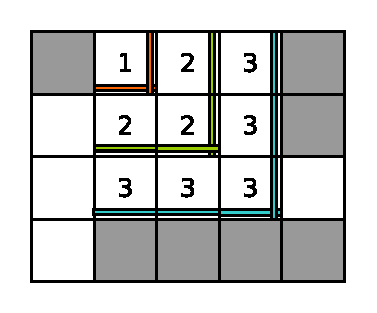
\includegraphics[]{sources/square_in_matrix/images/square_matrix_diagonal}
	\caption[Square in matrix - Brute-force diagonal]{This figure depicts the process of calculating the value of the side of the largest square having as a top-left corner cell $(0,1)$. Each cell is labeled with a number representing the step at which that cell is checked. Note that no cell is checked twice.}
\end{figure}


\lstinputlisting[language=c++, caption={C++ brute force solution using diagonal steps for solving the \textit{square in matrix} problem.  },label=list:square_in_matrix_diagonal]{sources/square_in_matrix/square_in_matrix_solution1.cpp}


\subsubsection{Dynamic programming}
Turns out that this problem can be solved faster than $O(N^3M)$ time and in this Section we will see
how with the help of Dynamic programming. The gist of the idea is based on the fact for any square
of size $k\times k$ having as bottom-left corner the cell $(x,y)$  has a top, top-left and left
subsquares of size $(k-1)\times (k-1)$. As an example see Figure
\ref{sources/square_in_matrix/images/square_decomposition} which shows a square of size $3\times 3$
decomoposed into $3$, $2\times 2$ subsquares.
\begin{figure}
	\centering
	\label{fig:square_in_matrix:squa_matrix_incremental}
	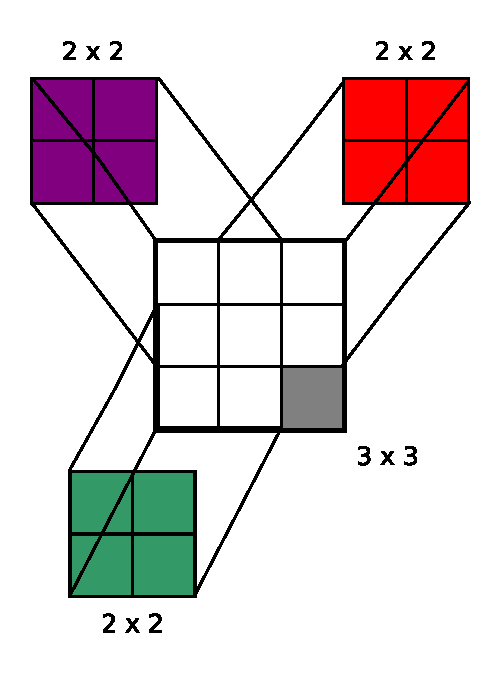
\includegraphics[width=\textwidth/2]{sources/square_in_matrix/images/square_decomposition}
	\caption[]{}
\end{figure}

Suppose $DP(i,j)$ contains is a function returning the size of the largest square having as $(i,j)$
as its bottom-right location. Clearly the values of DP for all cells belonging to the first row or
the first column are the same as in the input matrix (either 1 or 0 depending whether on the
corresponding value in the input matrix $M$). This is explained by the fact that a cell in the first
row or column lack one or more of the subsquares described above. For instance for a cell in the
first row, the top subsquare is missing (as there are no cells above it) and thus is impossible to
construct a square having a side larger than $1$ starting from it. For all the other (internal)
cells the value of $DP$ can be easily calculated by using the Equation
\ref{eq:square_in_matrix_DPformula}. The formula is basically stating that if we have a cell $(i,j)$
set to $1$ then, from it we can construct a larger square whose size depend on the size of the
smallest square of any of the neighboring subsquares.
\begin{equation}
	\label{eq:square_in_matrix_DPformula}
	DP(i,j) = min\{DP(i-1,j),DP(i-1,j-1), DP(i,j-1)\} +1
\end{equation}
Figure \ref{fig:square_in_matrix:square_DP_example} shows the idea above in practice. The value $2$ in $DP(1,3)$,$DP(1,2)$ and $DP(2,2)$  signifies that 
there is a square of size $2\times 2$ up to those cell in the original matrix. By combining those $3$ squares with the set cell at location $(2,3)$ 
we can build a larger square of size $3\times 3$.
Now consider the value of $DP(3,4)=3$. The entries for the neighboring cells $DP(3,4)=3$ and $DP(3,4)=3$ implies that a square of sie $3\times 3$ exists up to their indices, Butthe entry at location 
$DP(2,4)=1$ indicates that up to that cell only a square of size $1\times 1$ exists and this prevents cell $(3,4)$ to have a maximum square size larger than $2$.

\begin{figure}
	\centering
	\label{fig:square_in_matrix:square_matrix_diagonal}
	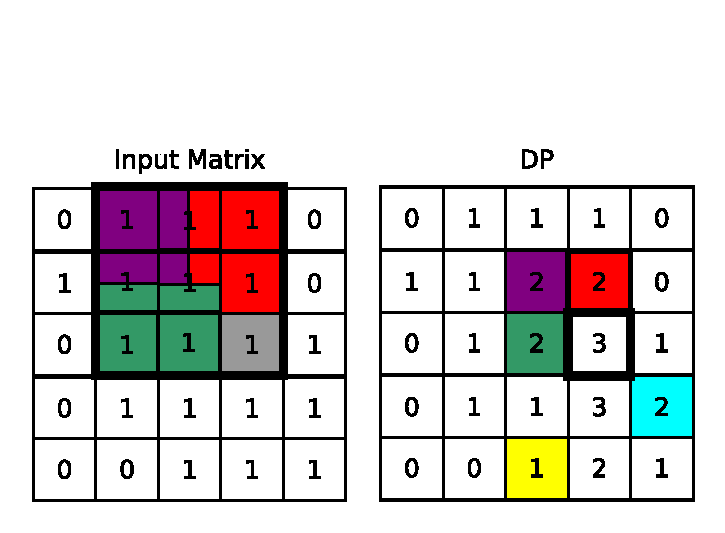
\includegraphics[]{sources/square_in_matrix/images/square_DP_example}
	\caption{ddddddddddddddddddd }
\end{figure}

The function DP in Equation \ref{eq:square_in_matrix_DPformula} is recursive and when drawing its recursion tree, as shown in 
Figure \ref{fig:square_in_matrix:recursiontree} (which depicts depicts part of the recursion tree for $DP(3,3)$),  we can easily see that:
\begin{itemize}
	\item the tree is complete and therefore has an exponential number of nodes.
	\item there are duplicate nodes.
\end{itemize} 
The number of possible unique function calls to DP is bounded by the values of its parameters which is far less than exponential. 
In-fact it is proportional to $N\time M$ (the size of the input matrix) as there are only $N$ possible value for $i$ and $M$ possible values for $j$ in $DP(i,j)$.
Therefore the only way for the recursion tree to have exponential number of nodes is for some of them to be duplicates. 
The problem then exposes the property of optimal substructure, because it can be solved by optimally solve smaller subproblems, and has overlapping subproblems. 
Therefore we can employ dynamic programming and solve each subproblem only once. 

\begin{figure}
	\centering
	\label{fig:square_in_matrix:recursiontree}
	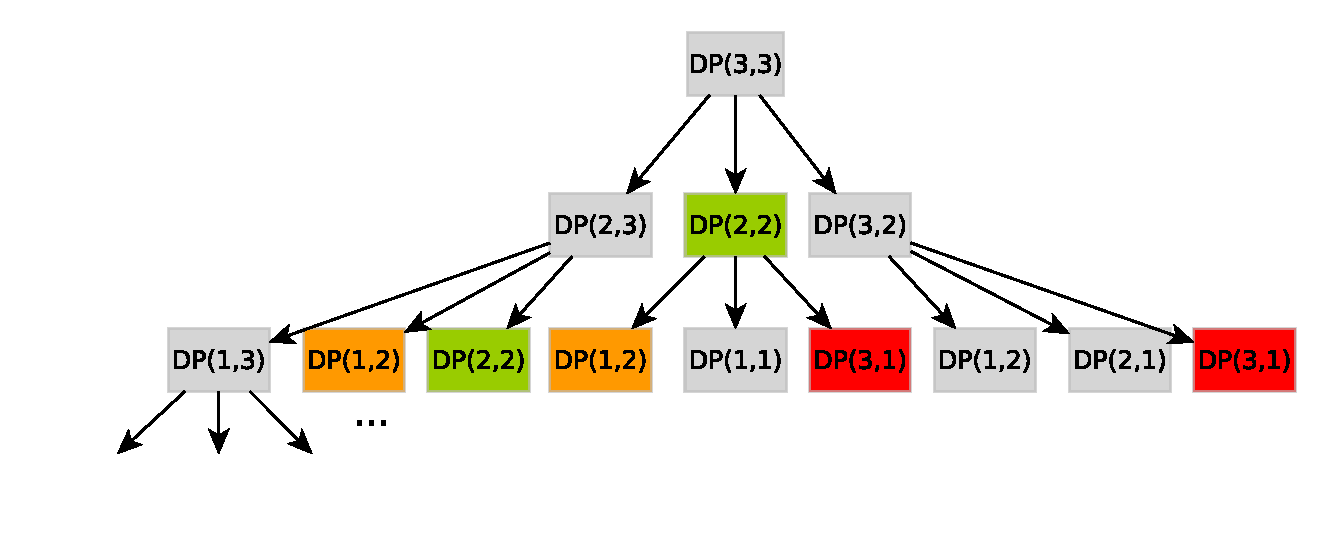
\includegraphics[width=\textwidth]{sources/square_in_matrix/images/recursiontree}
	\caption{ddddddddddddddddddd }
\end{figure}



